\documentclass[11pt,fullpage]{book}
\title{\textbf{~~~~~~~~~~~~~~~}\newline Chapter 3 - Likelihoods}
\author{}
\usepackage{natbib}
\usepackage{url,times}
\usepackage{graphicx}
\usepackage{epstopdf}
\usepackage{amsmath}
\usepackage[all]{xy}
\usepackage{pxfonts}
\usepackage{colortbl}
\usepackage{color}
\usepackage{subfigure}
\usepackage{gensymb}
\usepackage{ctable}
\usepackage[justification=centering]{caption}[2007/12/23]
\usepackage{longtable}
\usepackage{pstricks-add}
\usepackage{pstricks}
\usepackage{pst-func}
\usepackage{pst-math}

\setlength{\parindent}{0.0in}
\setlength{\parskip}{0.1in}
\maketitle

\begin{document}
\chapter{Likelihoods}
\section{Chapter Mission statement}
At the end of this chapter a reader will know how to choose an appropriate likelihood model for most situations. Further the reader will understand the basis behind maximum likelihood estimation.

Insert a graphic with the likelihood part of Bayes' formula circled.

\section{Chapter goals}
The starting point of the right hand side of the Bayesian formula is the likelihood function. This chapter will explain what is meant by a likelihood function, and why it is incorrect to view it as a probability for Bayesians. Further the choice over which likelihood to use for a given situation is often difficult to those unfamiliar with statistics. This chapter will provide practical guidance to likelihood choice, which should allow the student to be confident in their choice of model. As an important stepping stone to Bayesian estimation, this chapter will also explain how classical maximum likelihood estimation works. 

\section{What is a likelihood?}
In all statistical inference, we use an idealised, simplified, model to try to mimic relationships between real variables of interest. This model is then used to test hypotheses about the nature of the relationships between these variables. In Bayesian statistics the evidence for a particular hypothesis is summarised in posterior probability distributions. Bayes' magic rule tells us how we can compute this posterior probability distribution for a given parameter within a model, $\theta$:

\begin{equation}
P(\theta|data) = \frac{P(data|\theta)\times P(\theta)}{P(data)}
\end{equation}\label{eq:Likelihood_Bayes}

The first step to understanding this formula (so that we can ultimately use it!) is to understand what is meant by the numerator term, $P(data|\theta)$, which Bayesians call a Likelihood! Firstly, it's important to say that what we really mean by the numerator is:

\begin{equation}
P(data|\theta) = Probability(data|\theta,Model \; Choice)
\end{equation}\label{eq:Likelihood_simple}

What (\ref{eq:Likelihood_simple}) means is, what is the probability that we would have obtained the 'data', given (this is represented by the $|$ symbol) a particular value of $\theta$ and a particular choice of model. In other words, if our statistical model were true, and the value of the model's parameter were $\theta$, (\ref{eq:Likelihood_simple}) tells us the probability that we would have obtained our data. 

But what does this mean in simple, everyday language? Imagine that we flip a \textit{fair} coin. The most simple statistical model for coin flipping we can pick is to disregard the angle it was thrown at, as well as its height above the surface, along with any other details, and just pick the probability of the coin coming heads to be $\theta=\frac{1}{2}$. Furthermore, if a coin is thrown twice, we might choose to model the situation by assuming that the throwing technique is sufficiently similar between the two throws such that we can model each throw as independently having a probability of $\frac{1}{2}$. It's important to note that it is an assumption to forget about the throwing angle, as well as height of throw for each throw, and this forms part of our model of the situation. In this idealised model\footnote{Albeit in practicality, this is a pretty reasonable representation of the situation for most purposes.} of the situation the probability of the coin coming up as heads twice is simply $\frac{1}{2}\times\frac{1}{2}=\frac{1}{4}$. Written mathematically, this is simply the likelihood:

\begin{equation}
P(HH|\theta=\frac{1}{2},Simple\;Model) = \frac{1}{4}
\end{equation}\label{eq:Likelihood_fairCoin}

Hence, the likelihood simply summarises the possibility of obtaining a given set of data given a choice of model \textit{and} choice of the model's parameter(s). If we continue to assume that the probability of a head, $\theta$, is given by $\frac{1}{2}$, we can calculate the corresponding probabilities for all outcomes of throwing the coin twice. The most heads that can show up is 2, and the least being zero (if both flips come up tails). Figure \ref{fig:Likelihood_fairCoin} displays the probabilities for this model of the situation. The most likely number of heads to occur is 1, since this can occur in two different ways - either the first coin comes up heads, and the second is tails, or vice versa - whereas the other possibilities (all heads, or no heads) can each only occur in one way. The important thing to note however about figure \ref{fig:Likelihood_fairCoin} isn't the individual probabilities, it is that it represents as a whole a \textit{proper} probability distribution. What do we mean by this? Well, the individual event probabilities are all greater than 0 and less than 1, and when we sum the individual probabilities together we get 1 overall. So in the case where we assume a particular value for $\theta$, and keep it fixed there, the likelihood really is simply just a probability distribution. So, why do we bother changing its names from a 'probability' to a 'likelihood'? That is to be explained in the next section...

\begin{figure}
\centering
\scalebox{0.25} 
{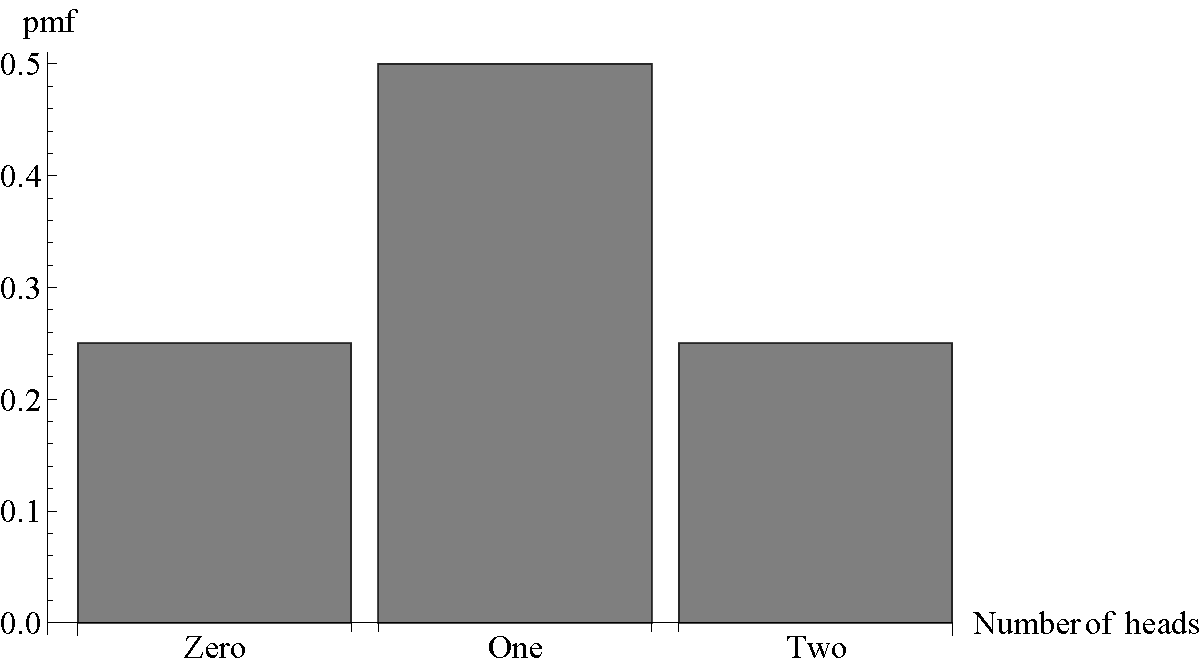
\includegraphics{Likelihood_fairCoin.png}}
\caption{Insert bar chart here of the number of heads along the x axis - 0,1,2 - and the associated probability of each of these outcomes as being the bar height - (1/4,1/2,1/4).}\label{fig:Likelihood_fairCoin}
\end{figure}

\section{Why is a likelihood not a probability for Bayesians?}
When we hold the parameters of our model fixed, as when we held the probability of an individual throw turning up heads to be $\theta=\frac{1}{2}$, we've reasoned that the first term of the numerator of Bayes' rule in (\ref{eq:Likelihood_Bayes}) really is simply a probability. So why don't we just keep calling it that, and forgo the introduction of this new word 'likelihood'? 

The reason is that in Bayesian inference, we \textit{don't} keep the parameters of our model fixed! In Bayesian analysis, it is the \textit{data} that is fixed, and we vary the parameters. Why do we do this? It is because a posterior probability distribution is a probability of a parameter in a model taking on a particular value, across a range of different parameter values. For the case of a coin, where we don't know the probability of a head beforehand, what we hope to get out is a probability distribution of the kind shown in figure \ref{fig:Likelihood_posteriorExample}. Notice that the x-axis in figure \ref{fig:Likelihood_posteriorExample} is the value of $\theta$ - the probability of a heads being obtained. In order to get this posterior probability, $P(\theta|data)$, for each value of theta, we use Bayes' rule in (\ref{eq:Likelihood_Bayes}). This means that for each \textit{different} value of $\theta$, we calculate the first part of the numerator which is $P(data|\theta)$; meaning that we calculate this across a range of $\theta$. If we assume that we have obtained two heads, and vary $\theta$ between 0 and 1 we can obtain the likelihood, which is shown in figure \ref{fig:Likelihood_coinLikelihood}. On first glances in might appear like \ref{fig:Likelihood_coinLikelihood} is a probability distribution, but first looks can be deceiving. 

\begin{figure}
\centering
\scalebox{0.25} 
{\includegraphics{Likelihood_posterior example.png}}
\caption{An example posterior distribution for the probability of a heads.}\label{fig:Likelihood_posteriorExample}
\end{figure}

\begin{figure}
\centering
\scalebox{0.25} 
{\includegraphics{Likelihood_posterior example.png}}
\caption{The x-axis here is theta, ranging between 0 and 1, assuming that one he}\label{fig:Likelihood_coinLikelihood}
\end{figure}

Checking off our necessary components of a probability distribution, we first note that all the values of the distribution in figure \ref{fig:Likelihood_coinLikelihood} are non-negative; which is what we require. However, if we look at the area underneath the curve in figure \ref{fig:Likelihood_coinLikelihood}, we find that it does not integrate to 1! Thus we have a violation of the second condition for a valid probability distribution. Hence, when we vary $\theta$ we find that, $P(data|\theta)$ is not a valid probability distribution!

Insert Bayesian box explanation.

\section{How to choose an appropriate likelihood}
\section{The subjectivity of model choice}
\section{Maximum likelihood - a short introduction}
\section{Chapter summary}


\end{document}